\section{Efekt \textit{overdrive}}

Pierwszym z~zaimplementowanych efektów dźwiękowych był tzw. przester (ang. \textit{overdrive}). Został on wybrany ze względu na możliwość relatywnie prostej realizacji. Schemat jego wyprowadzeń został przedstawiony na Rys. \ref{overdrive-structure}. Inkorporuje on siedem portów uniwersalnych dla wszystkich realizowanych efektów. Pierwsze dwa to \verb|clk| i~\verb|reset| opisane przy okazji omawiania modułów UART. Porty \verb|input data| oraz \verb|output data| stanowią wejście i~wyjście danych z~efektu\footnote{Dane traktowane są jako N-bitowe liczby w~formacie U2}. Przepisanie danych wejściowych do wewnętrznego bufora odbywa się po pojawieniu się stanu wysokiego na wejściu \verb|valid in|. Z~kolei na wyjściu \verb|valid out| logiczna jedynka ustawiana jest w~momencie wystawienia przetworzonych danych na czas trwania jednego cyklu zegarowego. Gdy wejście \verb|enable| znajduje się w~stanie niskim dane przepisywane są synchronicznie z~wejścia na wyjście bez wprowadzania zmian. Tak zaprojektowany interfejs pozwala - zgodnie z~założeniami - łączyć poszczególne efekty w~dowolnej koleności bez potrzeby ingerowania w~ich wewnętrzną strukturę.

\vspace{0.5cm}
\begin{figure}[ht]
    \centering
    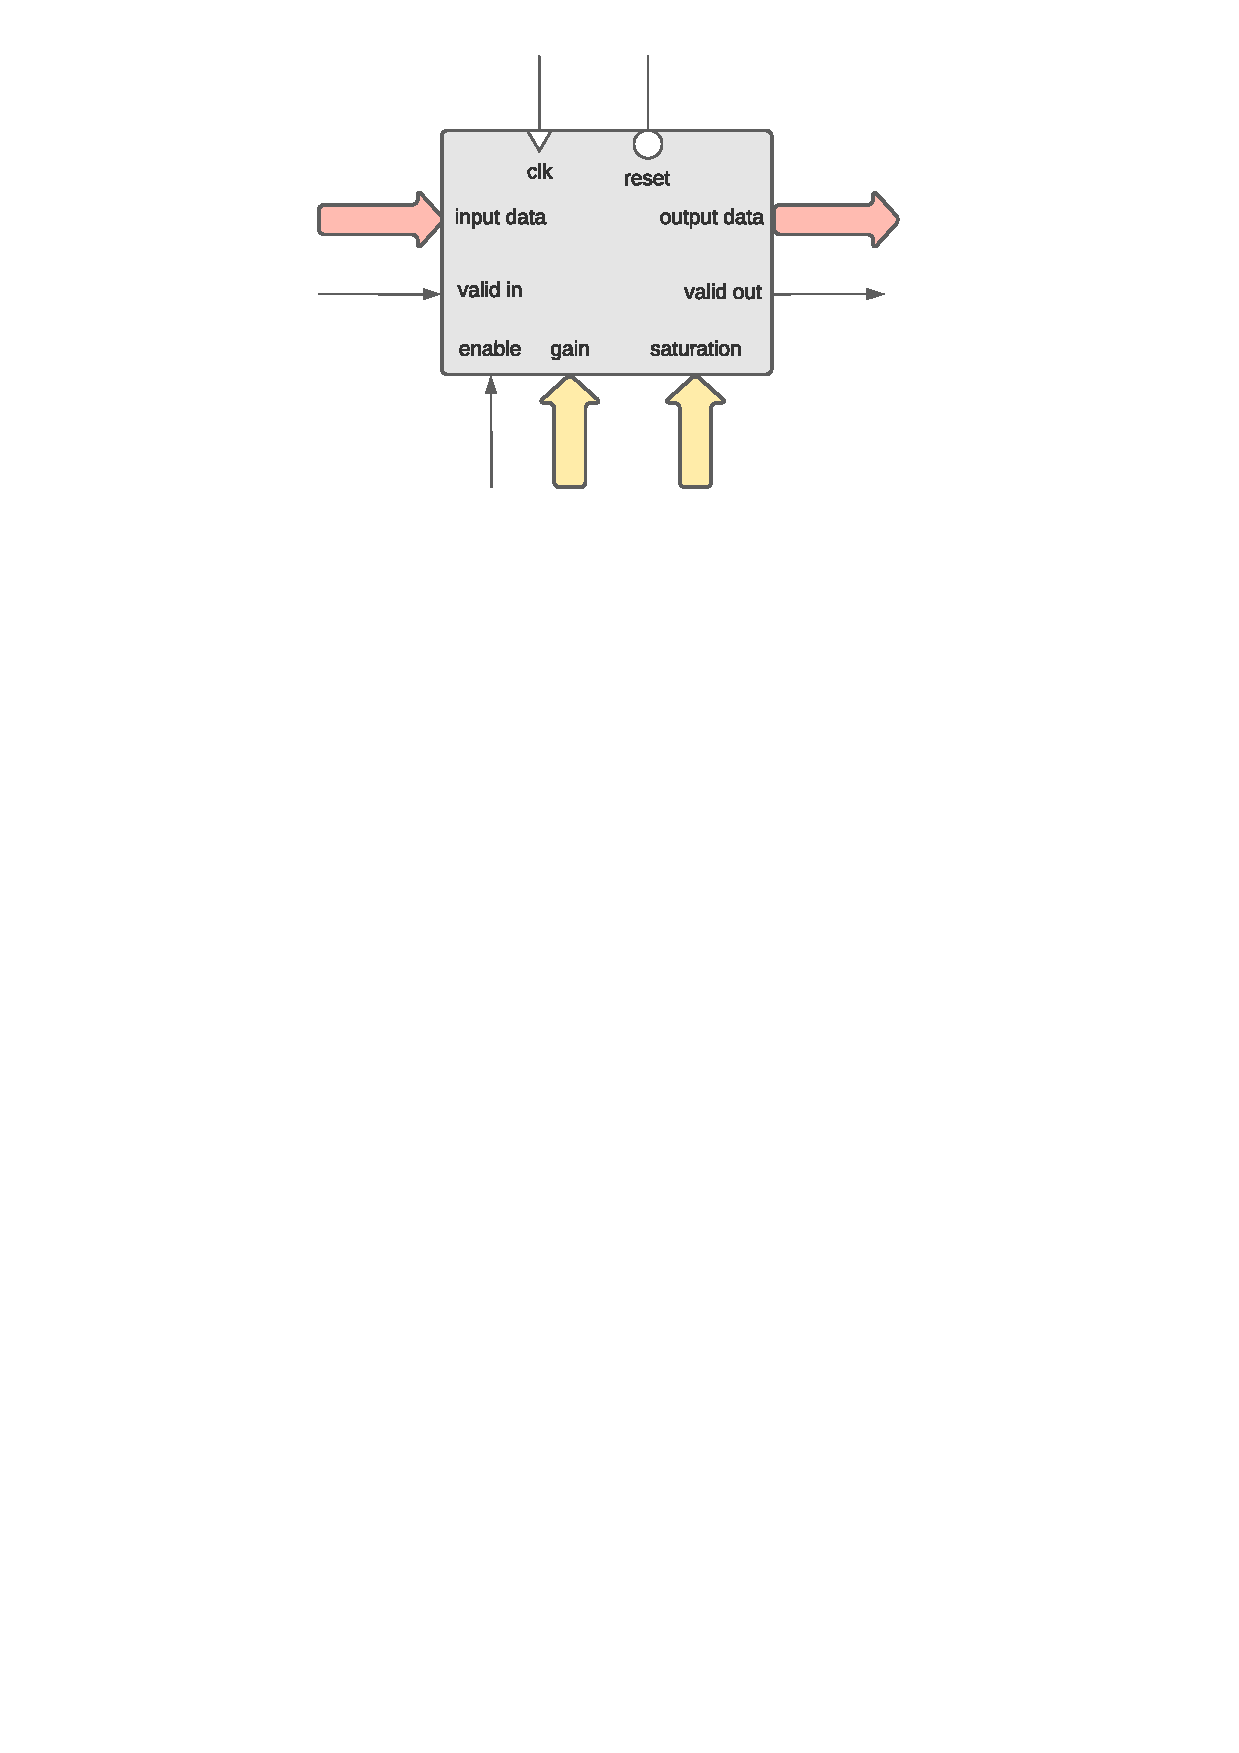
\includegraphics[scale=0.75]{img/diagrams/overdrive.pdf}
    \captionsetup{format=plain,justification=centering}
    \caption{Struktura wyprowadzeń bloku \textit{overdrive}}
    \label{overdrive-structure}
\end{figure}
\vspace{0.5cm}

Dwa dodatkowe porty wejściowe - \verb|gain| oraz \verb|saturation| - pozwalają dostosowywać parametry charakterstyczne filtra. Pierwszy z~nich określa czynnik przez jaki mnożona jest próbka wejściowa. Z~kolei drógi określa poziom obustronnego nasycenia wyniku mnożenia przed wystawieniem go na wyjście. Oba parametry traktowane są jako liczby bez znaku. Parametry modułu (\textit{generic}) pozwalają określić szerokość przetwarzanych próbek oraz wejścia \verb|gain|. Szerokość wejścia \verb|saturation| jest zawsze o~jeden bit mniejsza od szerokości próbek i~determinuje ograniczenie na \underline{wartość bezwzględną} próbki wyjściowej. Opcjonalnie możliwe jest też określenie przesunięcia bitowego (w~prawo) wyniku mnożenia przed podaniem go do bloku nasycenia. Pozwala to przeskalować efektywny zakres parametru \verb|gain| do obszaru wartości niecałkowitych.

Zasada działania modułu jest stosunkowo prosta. Po wykryciu stanu wysokiego na linii \verb|valid in| dane wejściowe, oraz parametry \verb|gain| i~\verb|saturation| przepisywane są do wewnętrznych buforów. Zawartość bufora danych i~wzmocnienia jest asynchronicznie mnożona (z~nasyceniem w~zakresie reprezentacji\footnote{W~ramach prac nad modułem \textit{overdrive} stworzona zostały cztery pomniejsze moduły DSP implementujące operacje dodawania i~mnożenia z~nasyceniem liczb z~i~bez znaku o~arbitralnej długości. Zostały one wykorzystane przy implementacji kolejnych efektów.}). W~następnym takcie zegara wynik mnożenia - opcjonalnie przesunięty o~skonfigurowaną liczbę bitów - zostaje nasycony w~granicach określonych przez bufor \verb|saturation| i~wystawiony na wyjście układu. Czas przetwarzania próbki wynosi \textbf{1~cyklu}. Jeżeli wejście \verb|enable| znajduje się w~stanie niskim, czas ten spada oczywiście do zera. 

Tak jak w~przypadku interfejsu analogowego stworzona została symulacja, której celem miała być jakościowa ocena pracy układu. Jej fragment ukazuje Rys. \ref{sim-overdrive}. Do testów wykorzystano falę sinusoidalną o~częstotliwości 440Hz reprezentowaną za pomoca próbek 16-bitowych. Szerokość wejścia \verb|gain| określono na $12$ bitów, przy czym wyjście z~układu mnożącego przesówane było o~$10$ bitów. Pozwala to na ustawianie wzmocnienia sygnału w~zakresie $[0,4)$. Jak widać na ukazanych przebiegach, włączenie modułu skutkuje wystąpieniem charakterystycznego ``przycinania'' próbek wejściowych.

\vspace{0.5cm}
\begin{figure}[ht]
    \centering
    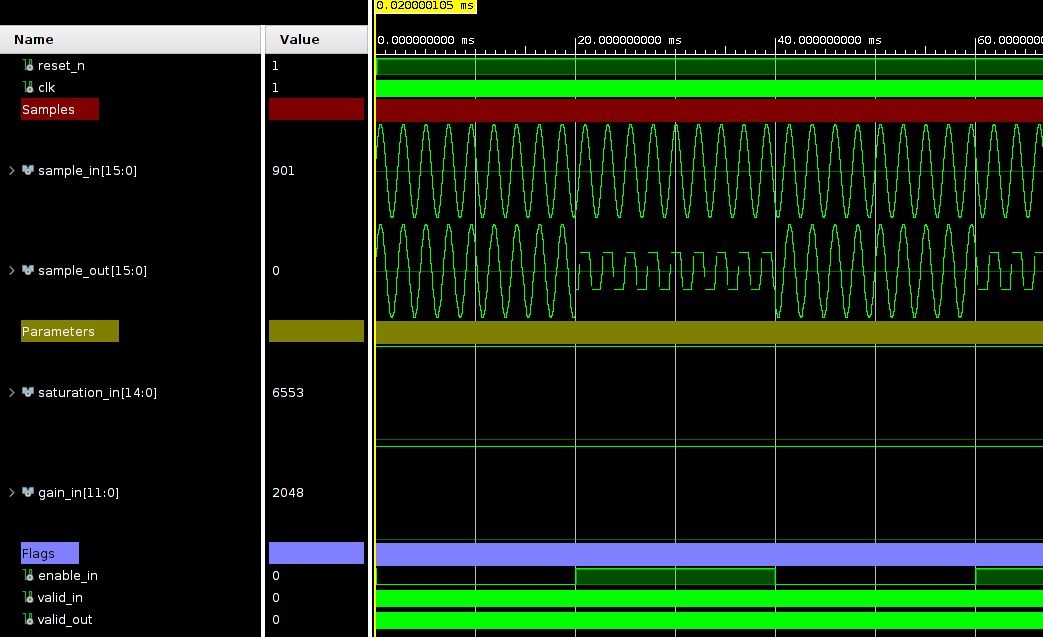
\includegraphics[width=\textwidth]{img/sim/overdrive_sim.png}
    \captionsetup{format=plain,justification=centering}
    \caption{Fragment symulacji działania efektu \textit{overdrive}}
    \label{sim-overdrive}
\end{figure}
\vspace{0.5cm}